\section{System Requirements}
\subsection{Personal Shopper}
\begin{enumerate}[label=SY-\arabic*]
    \item PSS shall enable a customers to register by requesting the 
    following fields:
    \begin{itemize}
        \item Name
        \item Last name
        \item Phone number
        \item Email
        \item Password
    \end{itemize}
    \item PSS shall enable customers to signup into the platform by using  
    authorized public OAuth implementation:
    \begin{itemize}
        \item Google
        \item Apple
    \end{itemize}

    \item PSS shall enable customers to login into the platform by 
    using email and password
    \item The PSS shall enable customers to login into the platform by using 
    authorized public OAuth implementation:
    \begin{itemize}
        \item Google
        \item Apple
    \end{itemize}

    \item PSS shall enable customers to close an existing session
    \item PSS shall display a list of all the available merchants
    \item PSS shall display what is the customer current location 
    inside a map
    \item When the customer is inside a merchant page, PSS shall enable the 
    customer to search a product
    \begin{itemize}
        \item PSS shall display a list of products that show the name, image 
        and short description that matches a search
    \end{itemize}
    \end{enumerate}
    \pagebreak
    \begin{enumerate}[resume, label=SY-\arabic*]
    \item PSS shall enable customers to add a product to the cart
    \item PSS shall enable customers to add their payment information 
    into the platform
    \item When the cart has one or more items, PSS shall permit the user to 
    create an order
    \item PSS shall permit customer to cancel an order
    \item PSS shall permit customer to confirm that they received an order
    \item If the customer forgets its password, PSS shall request to user to 
    enter its email address and shall an email with a temporary password
    \item If there is an issue with an order, PSS shall enable customers to 
    open an ticket about the order
    \item PSS shall enable user to send a message to the driver
    \item PSS shall display drivers information:
    \begin{itemize}
        \item Phone Number
        \item Name
        \item Profile Picture
    \end{itemize}
    \item PSS shall display the ETA from a pending order
    \begin{itemize}
        \item PSS shall display the ETA in terms of minutes
    \end{itemize}
    \item PSS shall display merchants information
    \begin{itemize}
        \item Name
        \item Phone 
        \item Email 
        \item Address
    \end{itemize}
\end{enumerate}
\pagebreak
\subsection{Personal Shopper Merchant}
\begin{enumerate}[resume, label=SY-\arabic*]
    \item PSMS shall enable merchants to login into the platform by 
    using email and password
    \item PSMS shall enable merchants to close an existing session
    \item PSMS shall enable merchants to add a product, by requesting the 
    following required fields.
    \begin{itemize}
        \item Name
        \item Description
        \item Picture
        \item Weight
    \end{itemize}
    \item PSMS shall enable merchants to update a selected product
    \item PSMS shall enable merchants to delete a selected product
    \begin{itemize}
        \item PSMS shall display a message dialog that request a confirmation 
        from the merchant
    \end{itemize}
    \item PSMS shall enable merchants to disable a product
    \item PSMS shall enable merchant to enable products that were 
    previously disabled
    \item If the merchant forgets its password, PSMS shall request to user 
    to enter its email address and shall an email with a temporary password
\end{enumerate}
\pagebreak
\subsection{Personal Shopper Driver}
\begin{enumerate}[resume, label=SY-\arabic*]
    \item  The PSDS shall enable merchants to login into the platform by 
    using email and password
    \item  The PSDS shall enable merchants to close an existing session
    \item  If the driver forgets its password, PSMS shall request to user to 
    enter its email address and shall an email with a temporary password
    \item  If the driver receives an order requests, PSDS shall request to 
    press a button with the title "Accept" to accept an order
    \item  If the driver receives an order requests, PSDS shall request to 
    press a button with the title "Decline" to accept an order
    \item  If the driver already accept an order, PSDS shall enabled the 
    user to decline the order
    \item  PSDS shall enable the driver to mark an order as delivered
	\item  If the driver mark an order as delivered, PSDS shall request the 
    user to take a picture of the delivery.
    \item  PSDS shall enable the driver to press a button that sends a signal 
    to PSSS that notifies to the customer that the driver it's on its 
    way to the merchant
    \item  PSDS shall enable the driver to press a button that sends a signal 
    to PSSS that notifies to the customer that the driver it's at the 
    merchant and it's working in the order
    \item  PSDS shall enable the driver to press a button that sends a signal 
    to PSSS that notifies the customer that the driver it's on its way to the 
    deliver the order to the customer
    \item  If the driver requires to reach out to the driver, PSDS shall 
    display the phone number of the customer
\end{enumerate}
\pagebreak
\begin{enumerate}[resume, label=SY-\arabic*]
    \item  PSDS shall display a list of all the orders that the drivers 
    performer in the last 30 days
    \item  PSDS shall display what is the driver current location inside a map
    \item  If the driver requires technical support, PSDS shall display a 
    technical support phone number
\end{enumerate}

\begin{figure}[!htb]
    \centering
    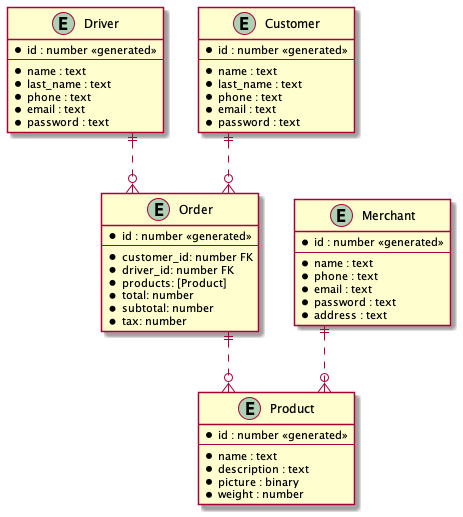
\includegraphics[scale=0.60]{data-model-diagram.png}
    \caption{Data Model Diagram}
\end{figure}